\documentclass[letterpaper]{article}
\usepackage[landscape, margin=0.2in]{geometry}
\usepackage{graphicx}
\usepackage{xcolor}
\usepackage{helvet}
\usepackage{url}
\usepackage{enumitem}
\usepackage{pagecolor}
\usepackage{array}
\usepackage{tabularx}
\usepackage{colortbl}
\usepackage{arydshln}
\usepackage{tikz}
\usepackage{qrcode}
\usepackage{eso-pic}
\usepackage{calc}

% Fold-line overlay at 1/3 and 2/3 of page width (landscape: 11" wide).
% Defined as a command so we can choose exactly which page(s) it's drawn on,
% rather than using \AddToShipoutPictureFG (which draws on every page).
\newcommand{\foldlines}{%
	\begin{tikzpicture}[remember picture, overlay]
		\draw[gray, dashed, line width=0.5pt]
		([xshift=3.666in] current page.south west) --
		([xshift=3.666in] current page.north west);
		\draw[gray, dashed, line width=0.5pt]
		([xshift=7.333in] current page.south west) --
		([xshift=7.333in] current page.north west);
	\end{tikzpicture}%
}

% Colors from OpenSaucePoster
\definecolor{posterblue}{RGB}{38, 61, 140}
\definecolor{posterrred}{RGB}{187, 31, 9}
\definecolor{posterorange}{RGB}{231, 164, 54}
\definecolor{posteryellow}{RGB}{242, 200, 61}
%e9ddafff
\definecolor{posterbeige}{RGB}{233, 221, 175}
\definecolor{posterlightblue}{RGB}{102, 102, 102}
\definecolor{posterdarkblue}{RGB}{0, 0, 255}
\definecolor{posterwhite}{RGB}{255, 255, 255}

% Set background and text colors
\pagecolor{posterbeige}
\color{posterblue}

\pagestyle{empty}
\setlength{\parindent}{0pt}
\setlength{\parskip}{0.1cm}

% Helper: wraps a panel's content so it only occupies 90% of the panel's
% width, centered, leaving a 5% margin on each side to account for folding.
\newcommand{\panelstart}{\begin{minipage}[t]{\linewidth}\centering\begin{minipage}[t]{0.9\linewidth}}
		\newcommand{\panelend}{\end{minipage}\end{minipage}}

% Icon helper: places a centered icon, sized to fit compactly next to text
% (kept small so the plugin list doesn't blow out the panel's height)
\newcommand{\pluginicon}[1]{%
	\raisebox{-0.15\baselineskip}{%
		\includegraphics[height=1.1\baselineskip]{#1}%
	}%
}

\begin{document}
	
	% \AddToShipoutPictureFG* only affects the very next page shipped out,
	% so the fold lines appear on page 1 (front) only, not page 2 (back/inside).
	\AddToShipoutPictureFG*{\foldlines}
	
	% ================== PAGE 1: FRONT ==================
	\begin{minipage}[c][\textheight][c]{\textwidth}
		\begin{center}
			\begin{tabular*}{\textwidth}{@{\extracolsep{\fill}}p{3.5in}p{3.5in}p{3.5in}}
				% PANEL 1: QUICK START & FEATURES
				\panelstart
				{\color{posterblue}\large\textbf{Key Features}}\\[0.2cm]
				\begin{itemize}[topsep=1pt, itemsep=1pt, leftmargin=*]
					\item Open Source with CC-1.0
					\item Easy Drag-And-Drop Workflow
					\item Local Application / No Internet
					\item Keep Files Local
					\item Non-Destructive workflow
					\item Advanced UI Features
					\begin{itemize}
						\item Timeline
						\item Feature Tree
						\item Focus to Clicked Point
					\end{itemize}
					\item Advanced CAD Features
					\begin{itemize}
						\item Fillet/Chamfer
						\item Convex Hull (Shrinkwrap)
						\item Intersection and Xor
						\item Extrude Surface
						\item Bend (Sweep surface)
						\item Hexagonal Pattern
						\item Radial patterns
					\end{itemize}
					\item Plugin support
					\\[0.05cm]
				\end{itemize}
				\vspace{-0.1cm}
				\noindent
				\begin{minipage}[t]{0.48\linewidth}
					\begin{itemize}[topsep=0pt, itemsep=0pt, leftmargin=1.6em]
						\item \pluginicon{Script-Tab-Blender.png} Blender
						\item \pluginicon{Script-Tab-OpenSCAD.png} OpenSCAD
						\item \pluginicon{Script-Tab-FreeCAD.png} FreeCAD
					\end{itemize}
				\end{minipage}%
				\hfill
				\begin{minipage}[t]{0.48\linewidth}
					\begin{itemize}[topsep=0pt, itemsep=0pt, leftmargin=1.6em]
						\item \pluginicon{build123d.png} Build123d
						\item \pluginicon{Script-Tab-SVG.png} Inkscape
						\item \pluginicon{eclipse.png} BowlerKernel
					\end{itemize}
				\end{minipage}
				\\[0.4cm]
				{\color{posterrred}\large\textbf{Community:}}\\[0.2cm]
				\begin{center}
					\begin{tabular*}{\linewidth}{@{\extracolsep{\fill}}cc}
						\small Active Discord Community & \small Active Github Project \\
						\qrcode[height=25mm]{https://discord.gg/fuJc3cbB7w} & \qrcode[height=25mm]{https://github.com/CommonWealthRobotics/CaDoodle-Application}
					\end{tabular*}
				\end{center}
				\panelend
				&
				% PANEL 2: DOWNLOADS & FAQs
				\panelstart
				{\color{posterblue}\large\textbf{FAQs}}\\[0.2cm]
				\footnotesize
				\textbf{Q: Is it free?} A: For Linux CaDoodle is free. Apple App Store or Microsoft Store versions require payment. Unsigned installers for all platforms are free.\\[0.1cm]
				\textbf{Q: Do I need to be online?} A: No, CaDoodle only needs internet access for updates.\\[0.1cm]
				\textbf{Q: What formats can I Export?} A: 3MF, STL, SVG, OBJ, Blender, FreeCAD\\[0.1cm]
				\textbf{Q: What if I only know TinkerCAD?} A: Everything learned in TinkerCAD translates to CaDoodle. Additional features can be learned over time, but aren't needed to get started.\\[0.1cm]
				\textbf{Q: What is Advanced Mode?} A: Adds more CAD tools and UI features. The Tinkercad-like workflow still works with extra capabilities.\\[0.1cm]
				\textbf{Q: If I bring my blender model in, will it mess it up?} A: No, CaDoodle is a non-destructive editor. It makes a copy when importing, then applies each step non-destructively.
				\\[0.3cm]
				
				{\color{posterrred}\large\textbf{Compatibility:}}\\[0.2cm]
				\textbf{Windows:} Standalone EXE, User Local, System-Wide\\[0.1cm]
				\textbf{Mac OS:} Apple Silicon (ARM), Intel (x86$_64$)\\[0.1cm]
				\textbf{Linux:} ARM/x86 AppImage, ARM/x86 Deb\\[0.1cm]
				\textbf{Chrome OS:} ARM/x86 Deb\\[0.1cm]
				\textbf{Stores:} Windows Store available
				\\[0.2cm]
				\small\textbf{Scan to Download:
					\\[0.3cm] cadoodlecad.com}\\[0.3cm]
				\begin{center}
					\qrcode[height=30mm]{https://cadoodlecad.com}
				\end{center}
				\panelend
				&
				% PANEL 3: COVER
				\panelstart
				\centering
				{\Huge\textbf{\color{posterblue}CADoodle}}\\[0.1cm]
				\rule{0.8\linewidth}{2pt}\\[0.1cm]
				{\large\textbf{\color{posterblue}FAQ Sheet}}\\[0.2cm]
				\includegraphics[width=0.7\linewidth]{OpenSaucePoster.pdf}\\[3.2cm]
				
				{\small\textbf{Made in Worcester, MA}}\\
				{\small\textbf{at Technocopia Makerspace}}\\[0.5cm]
				\panelend
			\end{tabular*}
		\end{center}
	\end{minipage}
	
	\newpage
	
	% ================== PAGE 2: BACK ==================
	% (no \AddToShipoutPictureFG* call here, so no fold lines on this page)
	\begin{minipage}[c][\textheight][c]{\textwidth}
		\begin{center}
			\begin{tabular*}{\textwidth}{@{\extracolsep{\fill}}p{3.5in}p{3.5in}p{3.5in}}
				% PANEL 1: SCREENSHOTS
				\panelstart
				{\color{posterblue}\large\textbf{Interface Preview}}\\[0.2cm]
				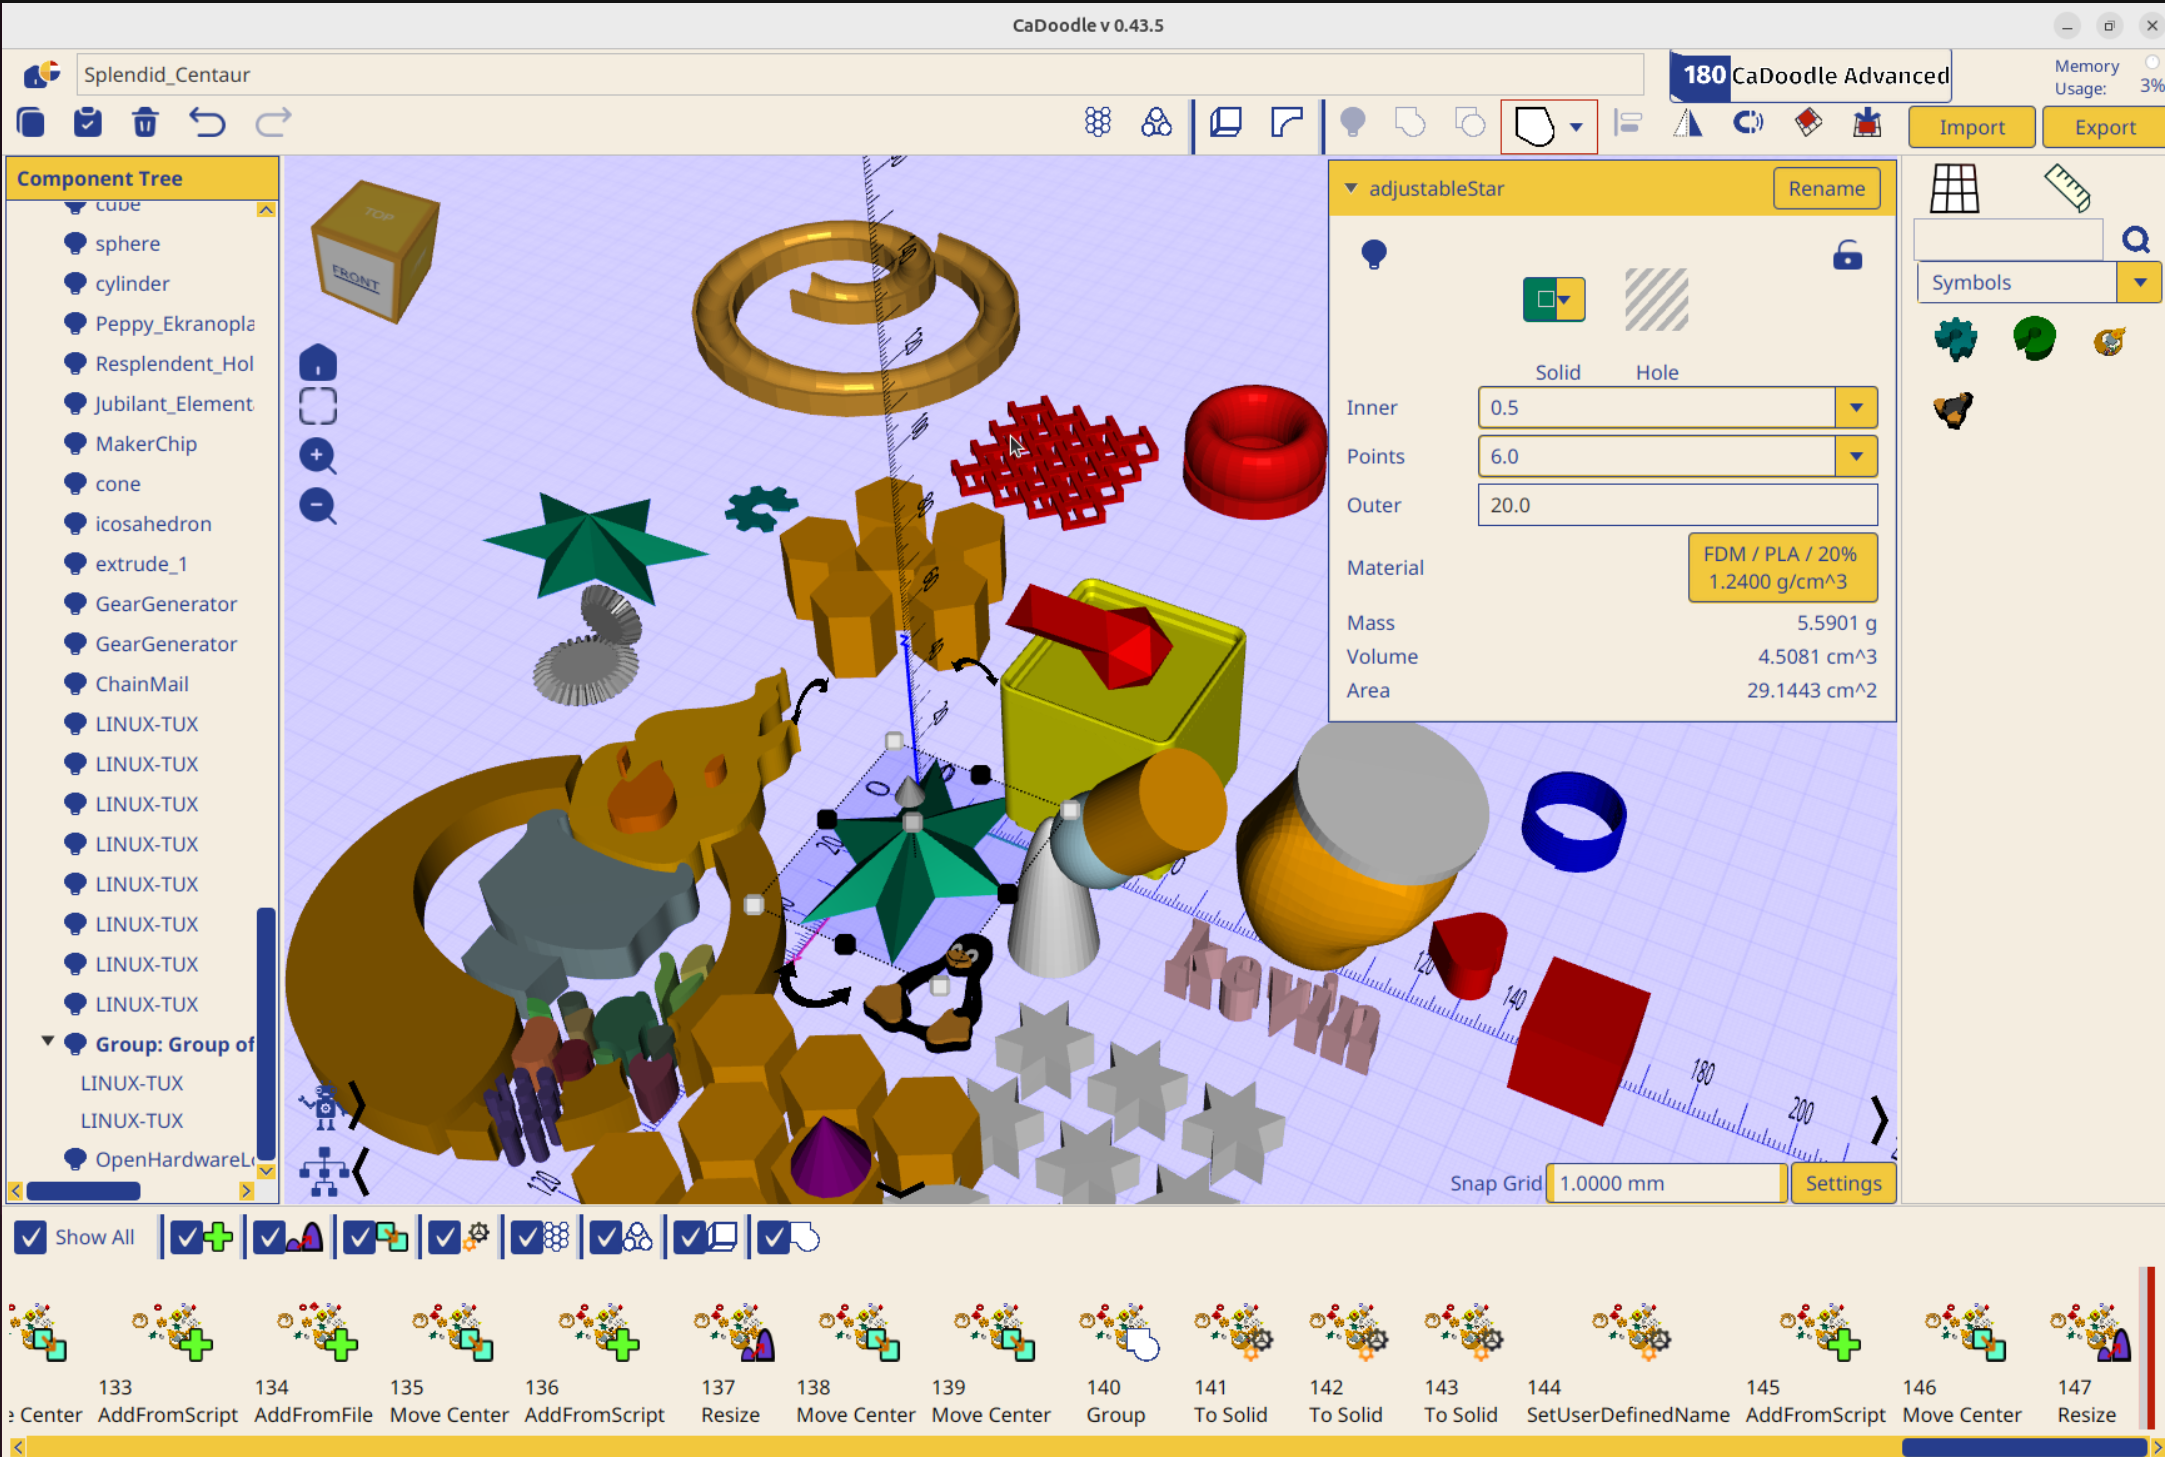
\includegraphics[width=0.9\linewidth]{CaDoodleScreenshot.png}\\[0.2cm]
				\small{\textbf{Main Interface}}\\[0.2cm]
				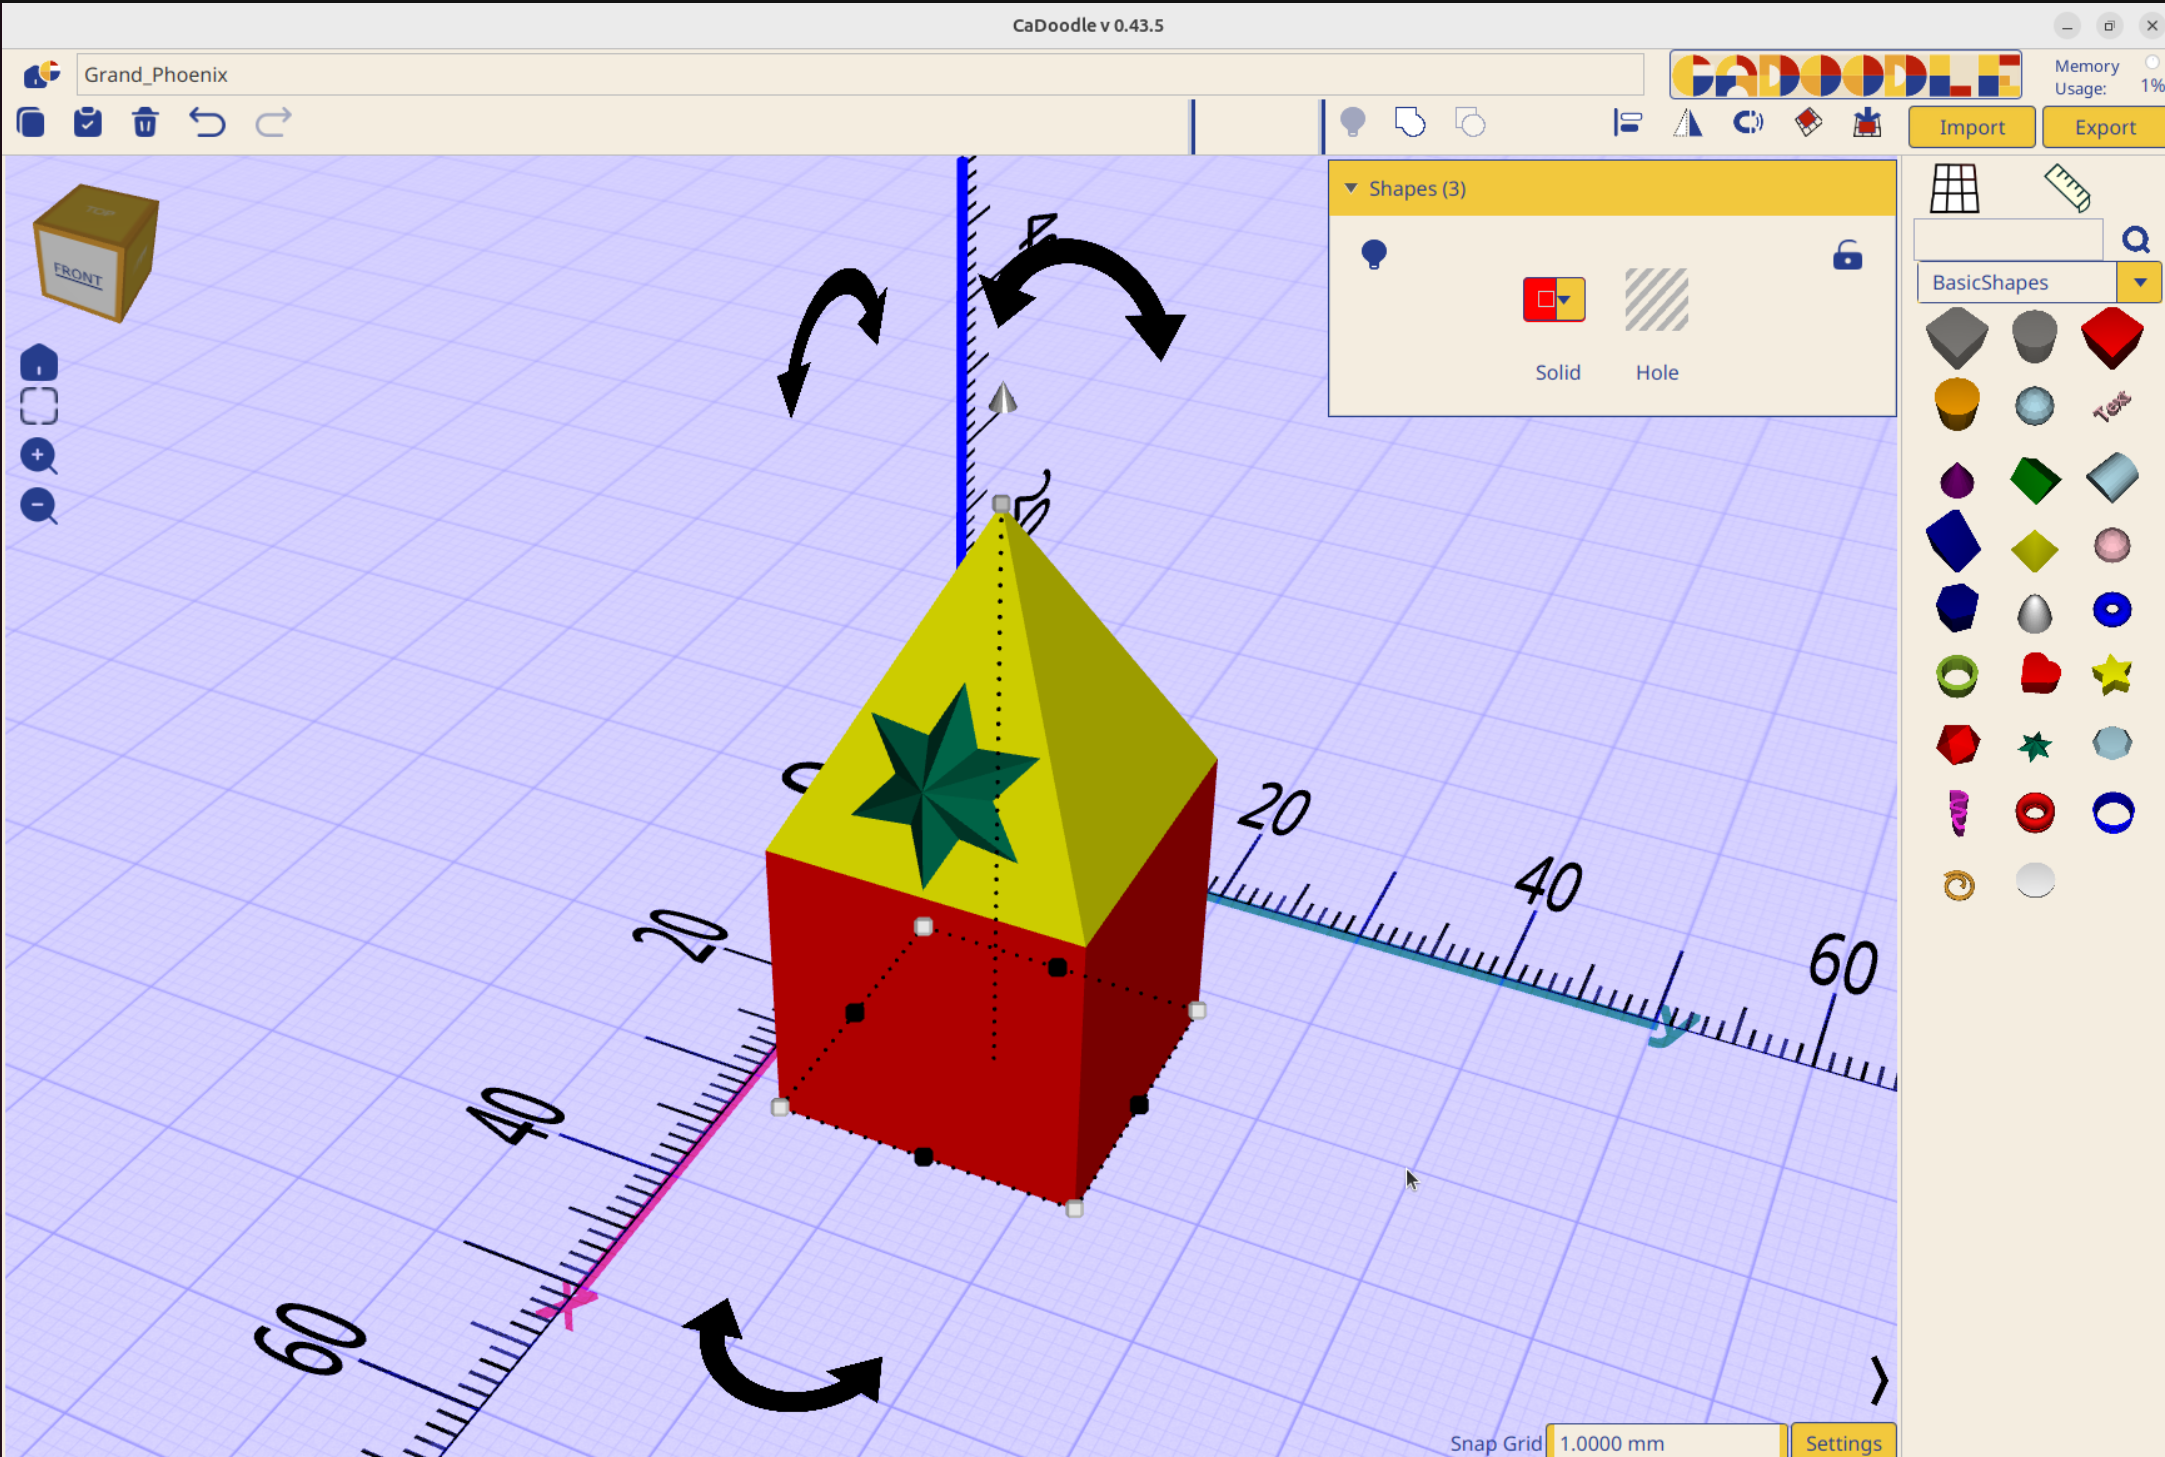
\includegraphics[width=0.9\linewidth]{BasicMode.png}\\[0.1cm]
				\small{\textbf{Basic Mode}}\\[0.2cm]
				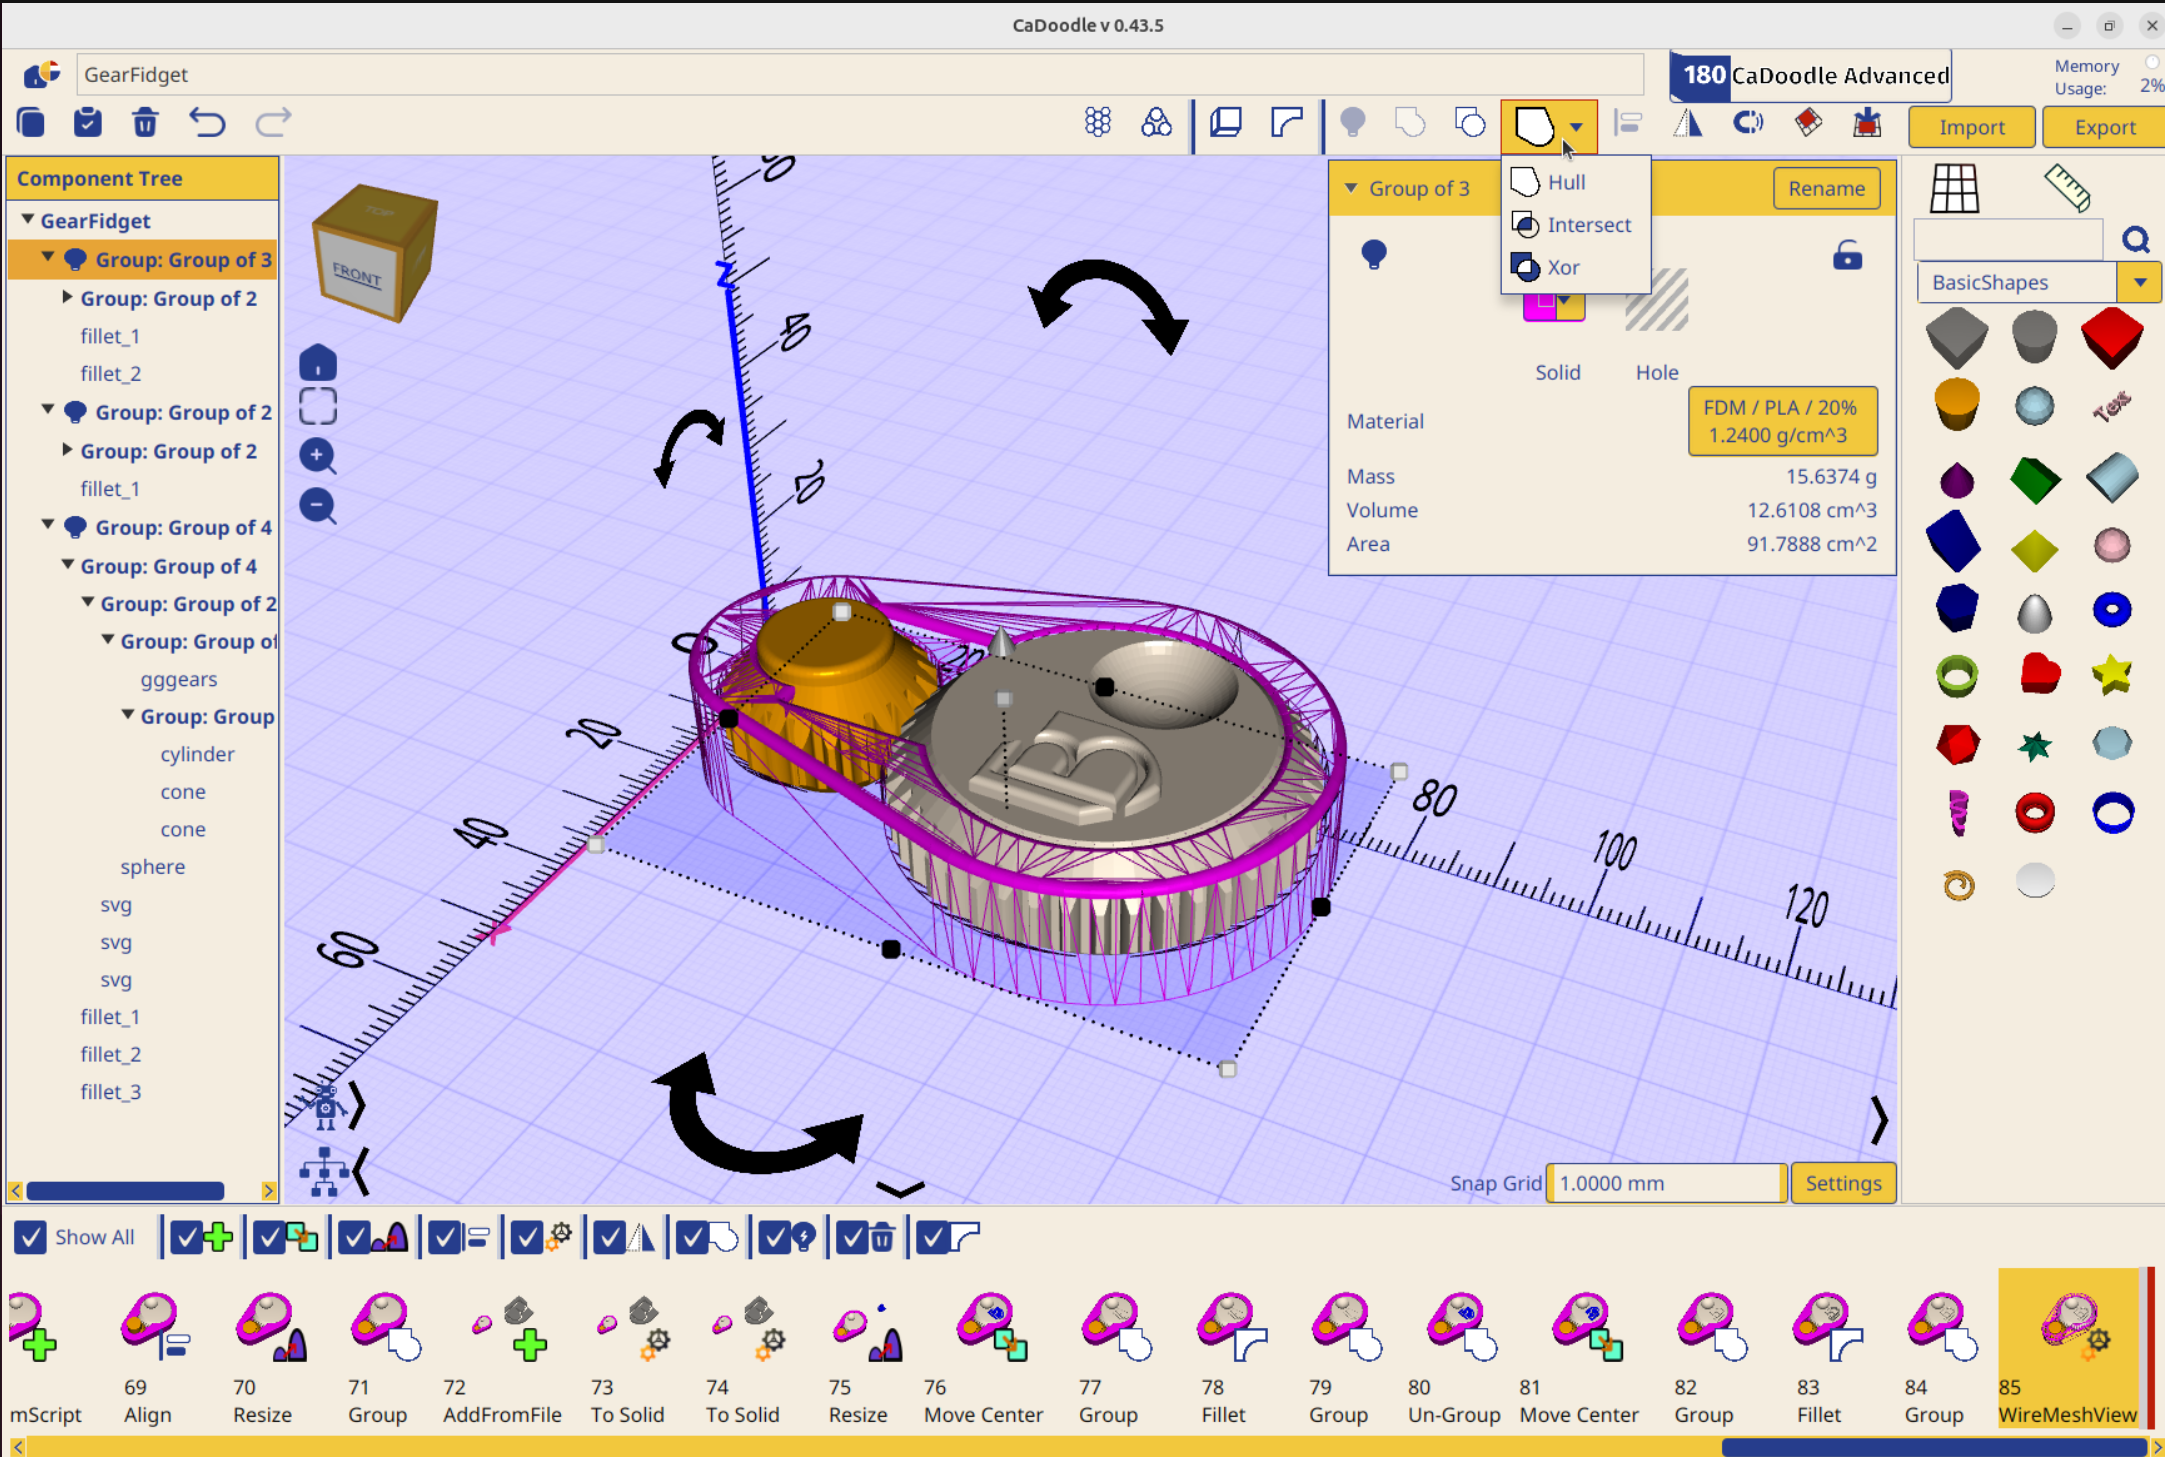
\includegraphics[width=0.9\linewidth]{AdvancedMode.png}\\[0.1cm]
				\small{\textbf{Advanced Mode}}\\[0.2cm]
				\panelend
				&
				% PANEL 2: BACK COVER
				\panelstart
				\raggedright
				\color{posterblue}\large\textbf{History}\\[0.2cm]
				\footnotesize
				\setlength{\parindent}{1em}
				In July 2024, the founder of CaDoodle, an elementary school technology teacher, began developing this project after years of using TinkerCAD with students as young as 1st grade.
				\\[0.2cm]
				The initial inspiration came from the need for an accessible, intuitive CAD tool that could engage young learners in creative design and problem-solving. However, the limitations of TinkerCAD became increasingly apparent: the proprietary nature of the source files meant students' work was trapped on Autodesk servers, inaccessible once the browser session ended.
				\\[0.2cm]
				A particularly memorable incident involved a complex student model that crashed the TinkerCAD website, resulting in total data loss with no recovery option. This experience highlighted the fragility of cloud-based design tools and the importance of local storage. Another pivotal moment occurred when a student wanted to continue her work during a long bus ride home—an hour each way—without internet access, demonstrating the impracticality of web-only solutions for students in rural or underserved areas.
				\\[0.2cm]
				The founder also became increasingly concerned about the pedagogical implications of teaching students skills mediated by a single corporation, fearing that this approach trained students to depend on proprietary ecosystems rather than fostering true computational thinking and creative autonomy.
				\\[0.2cm]
				These concerns led to the creation of CaDoodle: a locally installed, open-source CAD application that stores models on the user's own computer, uses open file formats, and runs offline without any internet connection. By July 2024, the project was under serious development, and by April 2025, it reached feature completeness for beta testing. Today, CaDoodle stands as a commitment to educational equity, digital sovereignty, and open-source collaboration.\\[0.2cm]
				
				\normalsize\textbf{Supporting CaDoodle Development}\\[0.2cm]
				
				\centering
				\qrcode[height=30mm]{https://venmo.com/u/Kevin-Harrington-17?txn=pay&amount=25&note=Donation} \quad
				\qrcode[height=30mm]{https://www.paypal.com/ncp/payment/FASUCA2FEFAJE}\\[0.1cm]
				\small{\textbf{Venmo}} \quad \small{\textbf{PayPal}}
				\panelend
				&
				% PANEL 3: EDUCATIONAL USE
				\panelstart
				{\color{posterblue}\large\textbf{Educational Use}}\\[0.2cm]
				\textbf{Schools:} No internet required, safe local storage\\[0.2cm]
				\textbf{Classroom Features:}\\
				\begin{itemize}[topsep=1pt, itemsep=1pt, leftmargin=*]
					\item No Accounts for easy on-boarding
					\item Support Fleet Deployment
					\item Simplified basic mode for beginners
					\item Timeline to fix students mistakes
					\item Advanced mode for experienced Students
					\item CAD tool grows with Students
					\item Free for Educators and Families
					\item Multiple language support
				\end{itemize}
				\vspace{0.2cm}
				{\color{posterrred}\large\textbf{Contact:}}\\[0.2cm]
				\small \textbf{Technocopia Makerspace}\\
				\small Worcester, MA\\[0.1cm]
				\small \url{support@cadoodlecad.com}\\[0.1cm]
				\small \textbf{Questions?} Scan to join:\\[0.1cm]
				\begin{center}
					\qrcode[height=30mm]{https://cadoodlecad.com/landing.html}
				\end{center}
				\panelend
			\end{tabular*}
		\end{center}
	\end{minipage}
	
\end{document}